%=========================================================
%               CLASSE DU DOCUMENT
%=========================================================
\documentclass[12pt,a4paper]{article}

%=========================================================
%         ENCODAGE ET POLICES DE CARACTÈRES
%=========================================================
\usepackage[utf8]{inputenc}    % Encodage UTF-8 (inutile avec XeLaTeX/LuaLaTeX)
\usepackage[T1]{fontenc}       % Meilleure gestion des caractères accentués
\usepackage{lmodern}           % Police Latin Modern
\usepackage{times}             % Police Times (à supprimer si tu préfères Latin Modern)

%=========================================================
%                MATHÉMATIQUES
%=========================================================
\usepackage{amsmath}           % Environnements mathématiques avancés
\usepackage{amssymb}           % Symboles mathématiques supplémentaires
\usepackage{amsfonts}          % Polices mathématiques
\usepackage{mathrsfs}          % Police calligraphique (\mathscr)
\usepackage{tkz-tab}           % Tableaux de signes et de variations
\everymath{\displaystyle}      % Affiche toutes les formules en style "display"

%=========================================================
%               MISE EN PAGE
%=========================================================
\usepackage[
    left=1cm,
    right=1cm,
    top=1cm,
    bottom=1.7cm
]{geometry}                    % Marges du document

\usepackage{multicol}          % Texte sur plusieurs colonnes
\usepackage{float}             % Placement précis des figures et tableaux

%=========================================================
%            TABLEAUX ET LISTES
%=========================================================
\usepackage{array}             % Colonnes de tableaux personnalisées
\usepackage{multirow}          % Fusion de lignes dans les tableaux
\usepackage{enumitem}          % Personnalisation des listes

%=========================================================
%            COULEURS ET BOÎTES
%=========================================================
\usepackage[most]{tcolorbox}   % Boîtes colorées très personnalisables
\tcbuselibrary{skins,hooks}    % Bibliothèques supplémentaires de tcolorbox

\usepackage{mdframed}          % Cadres autour de paragraphes
\usepackage{varwidth}          % Largeur automatique des boîtes

%=========================================================
%                DESSINS ET GRAPHIQUES
%=========================================================
\usepackage{tikz}              % Dessins vectoriels

\usetikzlibrary{
    arrows,
    shapes.geometric,
    fit,
    patterns
}

\usepackage{pgfplots}          % Tracés de fonctions et graphiques
\pgfplotsset{compat=1.15}

%=========================================================
%              LIENS HYPERTEXTES
%=========================================================
\usepackage[
    colorlinks=true,
    linkcolor=blue,
    urlcolor=blue,
    citecolor=blue
]{hyperref}

%=========================================================
%          ÉLÉMENTS EN ARRIÈRE-PLAN
%=========================================================
\usepackage{eso-pic}           % Ajout de filigranes ou d'éléments sur chaque page

%=========================================================
%              SYMBOLES DIVERS
%=========================================================
\usepackage{pifont}            % Symboles (✓, ✗, etc.)

%=========================================================
%      PERSONNALISATION DES LISTES NUMÉROTÉES
%=========================================================

\newcommand\circitem[1]{%
\tikz[baseline=(char.base)]{
\node[circle,draw=gray,fill=red!55,
minimum size=1.2em,inner sep=0] (char) {#1};}}

\newcommand\boxitem[1]{%
\tikz[baseline=(char.base)]{
\node[fill=cyan,
minimum size=1.2em,inner sep=0] (char) {#1};}}

\setlist[enumerate,1]{label=\protect\circitem{\arabic*}}
\setlist[enumerate,2]{label=\protect\boxitem{\alph*}}

%=========================================================
%            COMMANDES PERSONNALISÉES
%=========================================================

% Soulignement coloré
\newcommand{\myul}[2][black]{%
\setulcolor{#1}\ul{#2}\setulcolor{black}}

% Tabulation horizontale
\newcommand\tab[1][1cm]{\hspace*{#1}}

%=========================================================
%             COMPTEURS PERSONNALISÉS
%=========================================================

%---------- Exemple ----------
\newcounter{exemple}

\newcommand{\exemple}{%
\refstepcounter{exemple}
\textbf{\textcolor{orange}{Exemple \theexemple : }}
\ignorespaces}

%---------- Solution ----------
\newcounter{solution}

\newcommand{\solution}{%
\refstepcounter{solution}
\textbf{\textcolor{orange}{Solution \thesolution : }}
\ignorespaces}

%---------- Exercices ----------
\definecolor{myorange}{rgb}{1.0,0.8,0.0}

\newcounter{exerciceapp}

\newcommand{\exerciceapp}{%
\refstepcounter{exerciceapp}
\textbf{\textcolor{myorange}
{Exercice d'application \theexerciceapp : }}
\ignorespaces}

%---------- Corrections ----------
\newcounter{correction}

\newcommand{\correction}{%
\refstepcounter{correction}
\textbf{\textcolor{myorange}
{Correction \thecorrection : }}
\ignorespaces}

%---------- Remarques ----------
\definecolor{myorange1}{rgb}{1.0,1.0,0.0}

\newcounter{remarque}

\newcommand{\remarque}{%
\refstepcounter{remarque}
\textbf{\textcolor{myorange1}
{Remarque \theremarque : }}
\ignorespaces}

%=========================================================
%                 FILIGRANE
%=========================================================

\AddToShipoutPicture{
    \AtTextCenter{
        \makebox[0pt]{
            \rotatebox{45}{
                \textcolor[gray]{0.6}{
                    \fontsize{5cm}{5cm}\selectfont PGB
                }
            }
        }
    }
}

\begin{document}
% En-tête personnalisée
\begin{center}
    \Large\textbf{\underline{\textcolor{red}{Suites Numériques}}}\\[-0.1cm]
    \normalsize\textbf{Prof : M. BA} \hfill \textbf{Classe : TS2}\\[-0.1cm]
    \textbf{Année scolaire : 2025 -- 2026}
\end{center}

\section*{\underline{\textbf{\textcolor{red}{I. Généralités}}}}
\subsection*{\underline{\textbf{\textcolor{red}{1. Définition d'une suite}}}}
On appelle \textit{suite numérique} toute fonction définie de $\mathbb{N}$ ou d'une partie $E$ de $\mathbb{N}$ vers $\mathbb{R}$.

On note : $U : \mathbb{N} \rightarrow \mathbb{R}$ \\
\hspace*{3.3cm}$n \mapsto U_{n}$

Le réel $U_n$ est appelé  \textcolor{red}{\textit{terme général}} ou  \textcolor{red}{\textit{terme d'indice $n$}}.
L'ensemble des termes de la suite est noté $(U_n)$ et $n \in \mathbb{N}$ ou $(U_{n})n\in\mathbb{N}$.
\subsection*{\underline{\textbf{\textcolor{red}{2. Modes de définition d'une suite}}}}
\subsubsection*{\textcolor{red}{a) Suite définie explicitement}}

\textbf{\underline{ Definition }}

Lorsqu'une suite $(U_{n})$ est exprimée en fonction de $n$, alors on dit que la suite $(U_{n})$ est définie par une \textcolor{red}{\textit{formule explicite}} et on note $U_{n} = f(n)$.

\textbf{\underline{\exemple}}

Soit $(u_{n})$ et $(v_{n})$ des suites définies par : $u_{n}=2n^{2}+1$ $v_{n}=\dfrac{n^{2}-4}{2n} n\in\mathbb{N}^{*}$

Calculer 

$u_{0}$ ; $u_{10}$ ; $u_{50}$

$v_{1}$ ; $v_{10}$ ; $v_{50}$

\textbf{\underline{\solution}}

\subsubsection*{\textcolor{red}{b) Suite définie par récurrence}}

\textbf{\underline{ Definition }}
	
Lorsque la suite $(U_n)$ est définie par une relation entre $U_n$ et $U_{n+1}$, alors on dit que $(U_n)$ est définie par une \textcolor{red}{\textit{relation de récurrence}}.

	$$\left\lbrace\begin{array}{rcl} u_{0}& =& \alpha \\ u_{n+1}& =& 2u_{n}-3\end{array}\right.\;,\quad\left\lbrace\begin{array}{rcl} v_{1}& =& \alpha \\ v_{n+1}& =& f(v_{n})\end{array}\right.$$

\textbf{NB:} Par exemple, pour calculer $u_{p}$, il faudrait faire $p$ calculs successifs.	
	
\textbf{\underline{\exemple}}

\begin{equation*} 
    \begin{cases}
        u_{0}=2 \\
        U_{n + 1}=\frac{2U_n + 3}{U_n + 1}
    \end{cases}
\end{equation*}
Calculer les cinq premier termes de $u_{n}$.

\textbf{\underline{\solution}}
	
\textbf{\underline{\exerciceapp}}

Dans chacun des cas suivants, calculer les $6$ premiers termes de la suite $U_{n}$.
\begin{itemize}
\item[1.]$U_{n} = 7n^{2} - 5n + 2$, $n \in \mathbb{N}$.

\item[2.]$u_{n+1}=2u_{n}+3\text{ et }u_{0}=-1.$
\end{itemize}

\textbf{\underline{\correction}}


\subsection*{\underline{\textbf{\textcolor{red}{ 3. Représentation graphique des termes d'une suite }}}} 

\subsubsection*{\underline{\textbf{\textcolor{red}{ a) Suite explicite }}}} 

$-\ $ Si $u_{n}$ est définie de façon explicite ; $u_{n}=f(n)$ alors représenter graphiquement la suite $(u_{n})$ consiste à représenter dans un repère l'ensemble des points isolés $(n\;,\ u_{n}).$

$-\ $ On peut aussi représenter directement les valeurs des termes de la suite sur l'un des axes du repère.

\textbf{\underline{\exemple}}

Représenter les 6 premiers termes de la suite $(u_{n})$ définie par 

a) $u_{n}=\dfrac{n^{2}+1}{2n+3}$

\textbf{\underline{\solution}}\\
a)\\
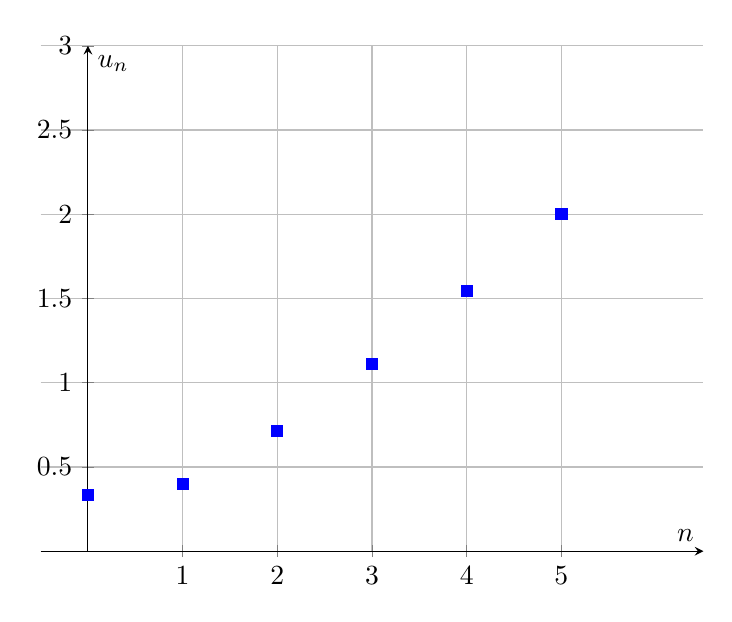
\begin{tikzpicture}
    \begin{axis}[
        axis lines = middle,
        xlabel = \( n \),
        ylabel = \( u_n \),
        ymin = 0,
        ymax = 3,
        xmin = -0.5,
        xmax = 6.5,
        xtick = {0, 1, 2, 3, 4, 5},
        ytick = {0, 0.5, 1, 1.5, 2, 2.5, 3},
        grid = both,
        width=10cm,
        height=8cm
    ]
        % Points de la suite
        \addplot[only marks, mark=square*, blue] coordinates {
            (0, 1/3)
            (1, 2/5)
            (2, 5/7)
            (3, 10/9)
            (4, 17/11)
            (5, 2)
        };
    \end{axis}
\end{tikzpicture}

b)\\
La suite \( u_n = 2n - 7 \) est représentée par les points \( (n, u_n) \) pour \( n = 0, 1, 2, 3, 4, 5 \).

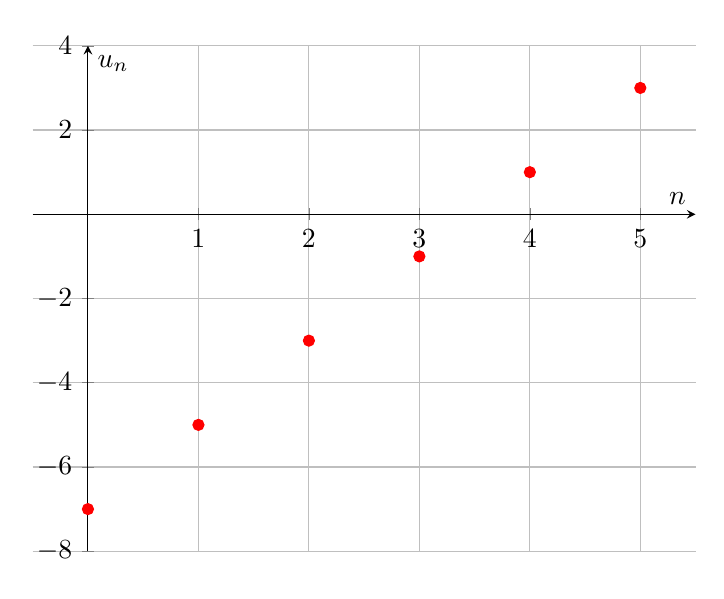
\begin{tikzpicture}
    \begin{axis}[
        axis lines = middle,
        xlabel = \( n \),
        ylabel = \( u_n \),
        ymin = -8,
        ymax = 4,
        xmin = -0.5,
        xmax = 5.5,
        xtick = {0, 1, 2, 3, 4, 5},
        ytick = {-8, -6, -4, -2, 0, 2, 4},
        grid = both,
        width=10cm,
        height=8cm
    ]
        % Points de la suite
        \addplot[only marks, mark=*, red] coordinates {
            (0, -7)
            (1, -5)
            (2, -3)
            (3, -1)
            (4, 1)
            (5, 3)
        };
    \end{axis}
\end{tikzpicture}

\subsubsection*{\underline{\textbf{\textcolor{red}{b) Suite définie par récurrence}}}} 

\[
\begin{cases}
u_0 = \alpha, \\
u_{n+1} = g(u_n),
\end{cases}
\]
où \( g \) est la fonction associée à la suite \((u_n)\).On trace \( C_g \), ainsi que la première bissectrice \( y = x \).  

Par une méthode graphique de projection, on construit les termes successifs de la suite \((u_n)\) en suivant les étapes suivantes :  

\begin{enumerate}
    \item On place le premier terme \( u_0 \) sur l’axe des abscisses.  
    \item On lit la valeur de \( u_1 = g(u_0) \) en projetant \( u_0 \) verticalement sur \( C_g \). Cette valeur se trouve sur l’axe des ordonnées.  
    \item On projette \( u_1 \) sur l’axe des abscisses à l’aide de la première bissectrice \( y = x \).  
    \item On utilise à nouveau la courbe \( C_g \) pour déterminer \( u_2 = g(u_1) \), en projetant \( u_1 \) verticalement sur \( C_g \).  
    \item On projette \( u_2 \) sur l’axe des abscisses via la première bissectrice.  
    \item On répète ce processus pour calculer les termes suivants \( u_3, u_4, \dots \).  
\end{enumerate}

Ce procédé, appelé *construction par itération graphique*, permet de visualiser l'évolution des termes de la suite \((u_n)\) et d'étudier son comportement (convergence, divergence ou oscillation).

\textbf{\underline{\exemple}}

Soit $(u_n)$ la suite définie par, $u_0=2$ et, pour tout $n\in\mathbb{N} \quad u_{n+1}=2\sqrt{u_{n}}$.

Construis les 6 premiers termes de $(u_n)$.

\textbf{\underline{\solution}}

Soit $f$ la fonction définie sur $[0;+\infty[$ par $f:x\mapsto 2\sqrt{x}$.
Ainsi, pour tout $n\in\mathbb{N}, u_{n+1}=f(u_{n})$ 

1.On trace $(\mathcal{C}_{f})$, la courbe représentation de la fonction $f$.

2.On trace la droite la d'équation $y=x$
\begin{center}
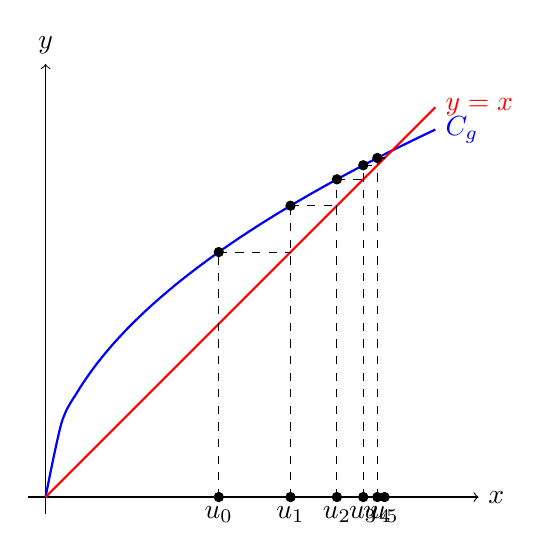
\begin{tikzpicture}[scale=1.1]

% Axes
\draw[->] (-0.2,0) -- (5,0) node[right] {$x$};
\draw[->] (0,-0.2) -- (0,5) node[above] {$y$};

% Courbe y = 2sqrt(x)
\draw[domain=0:4.5,smooth,variable=\x,blue,thick]
plot ({\x},{2*sqrt(\x)}) node[right] {$C_g$};

% Bissectrice
\draw[red,thick] (0,0) -- (4.5,4.5) node[right] {$y=x$};

% Valeur initiale
\def\u{2}

% Point initial sur l'axe
\filldraw[black] (\u,0) circle (1.5pt) node[below] {$u_0$};

% Construction des 6 termes : u0 à u5
\foreach \n in {1,2,3,4,5} {

    % Projection verticale vers la courbe
    \draw[dashed] (\u,0) -- (\u,{2*sqrt(\u)});
    
    % Point sur la courbe
    \filldraw[black] (\u,{2*sqrt(\u)}) circle (1.5pt);
    
    % Projection horizontale vers la bissectrice
    \draw[dashed] (\u,{2*sqrt(\u)}) -- ({2*sqrt(\u)},{2*sqrt(\u)});
    
    % Nouveau terme
    \pgfmathsetmacro\unew{2*sqrt(\u)}
    
    % Point sur l’axe des abscisses
    \filldraw[black] (\unew,0) circle (1.5pt)
    node[below] {$u_{\n}$};
    
    % Mise à jour
    \xdef\u{\unew}
}

\end{tikzpicture}
\end{center}
\textbf{\underline{\exerciceapp}}

b) $u_{n}=2n-7$

Soit \( (u_n)_{n \in \mathbb{N}} \) la suite définie par :
\[
\begin{cases} 
u_{n+1} = \sqrt{5u_{n}} + 1 \\ 
u_0 = 1. & 
\end{cases}
\]

\textbf{\underline{\correction}}

%=========================================================
\section*{\underline{\textbf{\textcolor{red}{II. Sens de variation d'une suite}}}}

%---------------------------------------------------------
\subsection*{\underline{\textbf{\textcolor{red}{1. Définitions}}}}

Soit $\left(u_n\right)$ une suite numérique.

\begin{itemize}
	\item La suite $\left(u_n\right)$ est \textbf{croissante} si :
	
	\(
	\forall n\in\mathbb{N},\quad u_{n+1}\geq u_n
	\)
	
	c'est-à-dire :
	\(
	u_{n+1}-u_n\geq 0.
	\)
	
	\item La suite $\left(u_n\right)$ est \textbf{décroissante} si :
	
	\(
	\forall n\in\mathbb{N},\quad u_{n+1}\leq u_n
	\)
	
	c'est-à-dire :
	\(
	u_{n+1}-u_n\leq 0.
	\)
	
	\item La suite $\left(u_n\right)$ est \textbf{constante} si :
	
	\(
	\forall n\in\mathbb{N},\quad u_{n+1}=u_n.
	\)
\end{itemize}


\medskip

\textbf{Étudier le sens de variation d'une suite} $\left(u_n\right)$
consiste à déterminer si elle est croissante, décroissante ou constante.


%---------------------------------------------------------
\subsection*{\underline{\textbf{\textcolor{red}{2. Méthodes d'étude du sens de variation}}}}


%---------------------------------------------------------
\subsubsection*{\textcolor{red}{a) Méthode de la différence}}

On étudie le signe de la différence :
\(
u_{n+1}-u_n.
\)

\begin{itemize}
	\item Si :
	\(
	u_{n+1}-u_n\geq0,
	\)
	alors la suite $\left(u_n\right)$ est croissante.
	
	\item Si :
	\(
	u_{n+1}-u_n\leq0,
	\)
	alors la suite $\left(u_n\right)$ est décroissante.
\end{itemize}

\medskip

Cette méthode est la plus générale et peut être utilisée dans la majorité
des situations.


%---------------------------------------------------------
\subsubsection*{\textcolor{red}{b) Méthode du quotient}}

Lorsque les termes de la suite sont strictement positifs :
\(
u_n>0,
\)

on peut étudier le quotient :
\(
\frac{u_{n+1}}{u_n}.
\)

\begin{itemize}
	\item Si :
	\(
	\frac{u_{n+1}}{u_n}\geq1,
	\)
	alors $\left(u_n\right)$ est croissante.
	
	\item Si :
	\(
	\frac{u_{n+1}}{u_n}\leq1,
	\)
	alors $\left(u_n\right)$ est décroissante.
\end{itemize}

\textbf{Remarque :} Cette méthode nécessite obligatoirement que
$u_n>0$.


%---------------------------------------------------------
\subsubsection*{\textcolor{red}{c) Méthode par une fonction associée}}

Si la suite est définie par :
\(
u_n=f(n),
\)

où $f$ est une fonction définie sur un intervalle contenant $\mathbb{N}$,
on peut étudier les variations de $f$.

\medskip

Le sens de variation de la fonction $f$ permet alors de conclure sur
celui de la suite $\left(u_n\right)$.


%---------------------------------------------------------
\subsubsection*{\textcolor{red}{d) Méthode par récurrence}}

Dans certains cas, il est difficile d'étudier directement
$u_{n+1}-u_n$.

On peut alors démontrer par récurrence une propriété du type :

\(
u_{n+1}\geq u_n
\)

ou

\(
u_{n+1}\leq u_n.
\)


%---------------------------------------------------------
\subsection*{\underline{\textbf{\textcolor{red}{3. Méthode pratique}}}}

Pour étudier le sens de variation d'une suite, on choisit généralement :

\begin{itemize}
	\item \textbf{La différence} $u_{n+1}-u_n$ : méthode la plus utilisée ;
	
	\item \textbf{Le quotient} $\dfrac{u_{n+1}}{u_n}$ :
	 lorsque les termes sont positifs ;
	
	\item \textbf{La fonction associée} :
	 lorsque $u_n=f(n)$ ;
	
	\item \textbf{La récurrence} :
	 lorsque la suite est définie par une relation de récurrence.
\end{itemize}

\exerciceapp

On considère les suites $\left(u_n\right)$ définies pour tout entier naturel
$n$ par :

\begin{enumerate}
    \item 
    \[
    u_n=n^2+3n+1
    \]
    
    \begin{enumerate}
        \item Étudier le sens de variation de la suite $\left(u_n\right)$ à l'aide de la différence $u_{n+1}-u_n$.
        \item En déduire le minimum de la suite.
    \end{enumerate}

    \item 
    \[
    v_n=2^n
    \]
    
    \begin{enumerate}
        \item Étudier le sens de variation de la suite $\left(v_n\right)$ en utilisant la méthode du quotient.
    \end{enumerate}

    \item 
    \[
    w_n=\frac{n}{n+1}
    \]
    
    \begin{enumerate}
        \item Étudier le sens de variation de la suite $\left(w_n\right)$ à l'aide de la différence.
    \end{enumerate}

    \item 
    Soit la suite $\left(t_n\right)$ définie par :
    
    \[
    t_0=1,\qquad t_{n+1}=\frac{1}{2}(t_n+3)
    \]
    
    \begin{enumerate}
        \item Calculer les premiers termes de la suite.
        \item Montrer que :
        \[
        t_{n+1}-t_n=\frac{1}{2}(3-t_n).
        \]
        \item En supposant que $t_n<3$ pour tout $n$, étudier le sens de variation de $\left(t_n\right)$.
    \end{enumerate}
\end{enumerate}


\end{document}